%%%%%%%%%%%%%%%%%%%%%%%%%%%%%%%%%%%%%%%%%%%%%%%%%%%%%%%%%%%%%%%%%%%%%%%%
\section{Results} 
\label{sec:results}
%%%%%%%%%%%%%%%%%%%%%%%%%%%%%%%%%%%%%%%%%%%%%%%%%%%%%%%%%%%%%%%%%%%%%%%%

To compare SSD performance versus YOLO performance on Jetson TX1, we used their supplied applications for object detection on image files. We profiled both algorithms while they analyze 600 images from MSCOCO dataset \cite{mscoco}. The measured time is the actual kernel execution time, we do not take into consideration the CPU execution time. We made three comparison between the two algorithms: when both run on (1) CPU, (2) GPU without cuDNN, and (3) GPU with cuDNN\footnotemark.

\footnotetext{The NVIDIA CUDA Deep Neural Network library (cuDNN) is a GPU-accelerated library of primitives for deep neural networks. cuDNN provides highly tuned implementations for standard routines such as forward and backward convolution, pooling, normalization, and activation layers.}

Figure \ref{fig:t_exec} shows the execution time of both SSD and YOLO for each of the options described above.
Not surprisingly, running object detection algorithms on a CPU is not as efficient as running them on a GPU. The GPU built-in parallelism is advantageous for such algorithms. The CPU performance is in order of magnitude worse than its GPU counterpart. 

The variation in the execution time when running with and without cuDNN is due to different implementations. YOLO without cuDNN performs better than with cuDNN. On the other hand, SSD with cuDNN performs better than without cuDNN.

SSD and YOLO performance is almost identical when compiled with cuDNN. It is interesting, since SSD claims to have better performance than YOLO \cite{liu2016ssd}. SSD was benchmarked with NVIDIA Titan X, which has a newer microarchitecture (Pascal vs. Maxwell), 14x more CUDA cores (3584 vs. 256), greater capacity faster memory (12GB GDDR5X vs. 4GB shared LPDDR4), and higher frequency. When system resources are scarce, the performance gains achieved by the algorithm are insignificant, therefore we do not see any major performance advantage towards SSD.

\begin{figure}[h]
	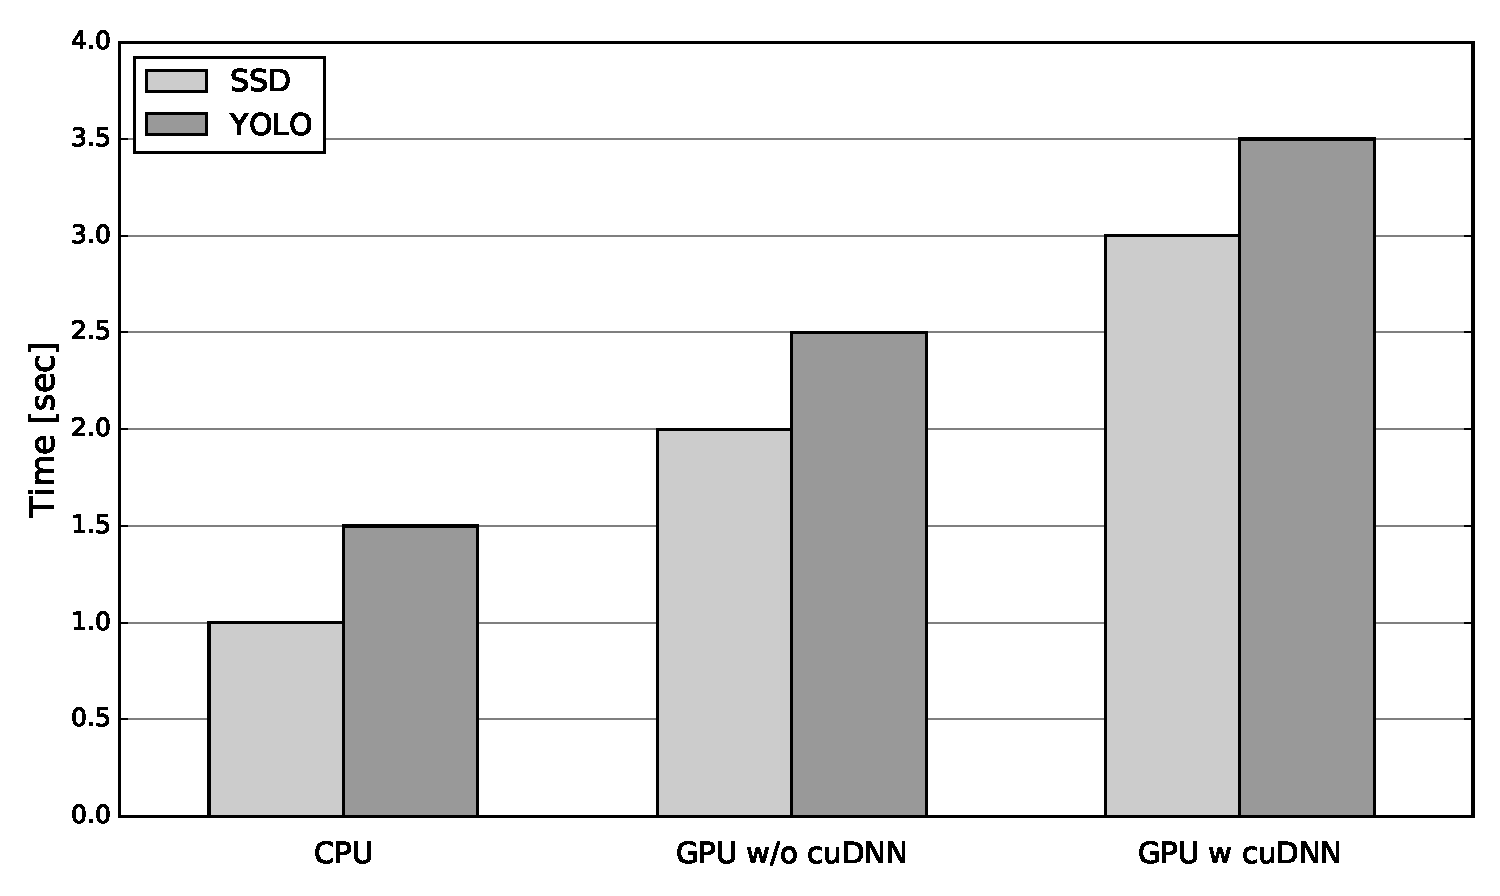
\includegraphics[width=0.48\textwidth]{./imgs/t_exec.pdf}
	\caption{Comparison of SSD and YOLO performance in different modes; CPU execution time is in order of magnitude worse than the GPU execution time}
	\label{fig:t_exec}
\end{figure}

SSD and YOLO are also packed with a web-camera demo. The original FPS readings used in the demo code are wrong, since they are based on the CPU execution time on the on the GPU execution time, therefore, the original, incorrect readings, are higher. After fixing the source code, we have measured 3.8FPS when using SSD and 4.7FPS when using YOLO. We ran the demo when both SSD and YOLO are compiled with cuDNN, and after running the \textit{jetson\_clocks.sh} script (see Section \ref{sec:installation}).

YOLO 4.7FPS fits the 200msec measurement shown in Figure \ref{fig:t_exec} ($200msec [sec/frame] = 5[frame/sec]$). The slightly lower FPS measured is due to the software overheads (e.g., fetching the images, operating system, etc.).

SSD web-camera FPS is lower since the code that runs it is synchronous, meaning after an image was acquired from the web-camera it is inserted to the the neural network. YOLO web-camera demo, on the other hand, is implemented asynchronously with a double buffer, meaning that while an image is analyzed in the neural network, an image is acquired. Consequently, the acquiring time is saved. 

\begin{figure}[h]
	\subfloat[SSD: 3.8FPS]{
		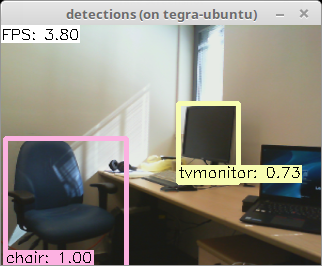
\includegraphics[width=0.23\textwidth]{./imgs/ssd_38fps.png}
		\label{fig:cam:ssd}
	}
	\subfloat[YOLO: 4.7FPS]{
		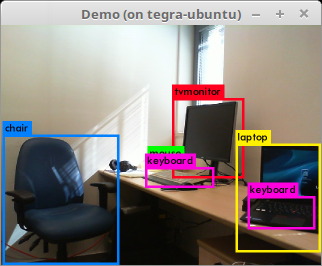
\includegraphics[width=0.23\textwidth]{./imgs/yolo_47fps.png}
		\label{fig:cam:yolo}
	}
	\caption{Object detection with SSD and YOLO using the the web-camera demo}
	\label{fig:cam}
\end{figure}